%-----appendices
\begin{appendices}
\noappendicestocpagenum
\addappheadtotoc
\chapter{Checklist for cooldown}
%-----appendices
\label{appendix:checklist-for-cooldown}

The preparation for a cooldown is not optional.  The checklist in Figure \ref{fig:checklist} should be gone through and double checked before LHe is ordered.


The entire group should be made aware if something on the checklist is not satisfied when LHe is ordered.  All subsequent procedures and operations in the Practical Operation (Chapter \ref{chapter:practical-op}) then need to be reviewed for potential modification to accommodate the missing prep.

\begin{figure}[!htbp]
 \centering
 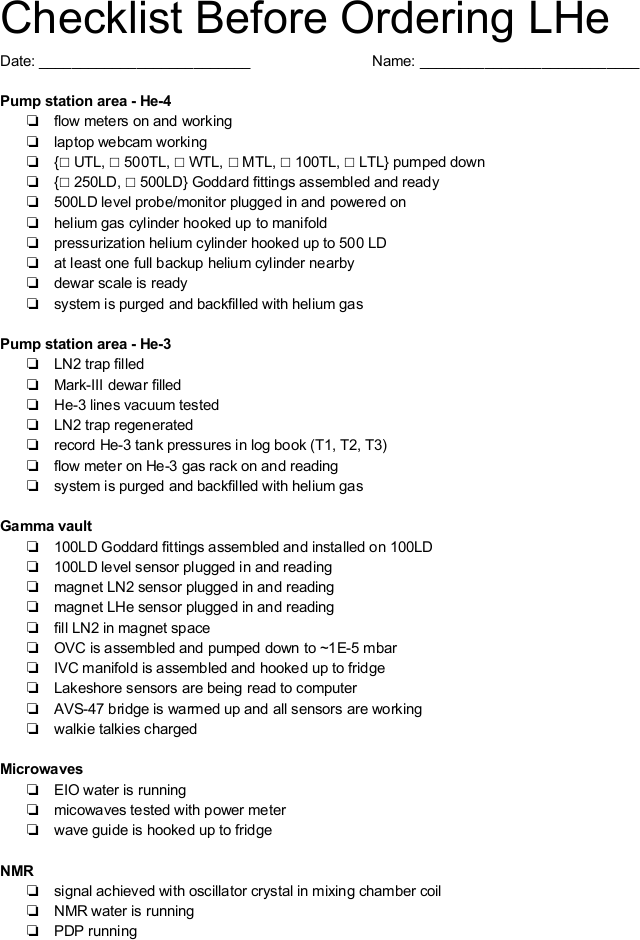
\includegraphics[height=.95\textheight]{./docs/cooldown-checklist.png}
 % cooldown-checklist.pdf: 0x0 pixel, 0dpi, 0.00x0.00 cm, bb=
 \caption{Checklist.}
 \label{fig:checklist}
\end{figure}



\chapter{SLPM Conversion}
\label{appendix:slpm-conversion}
Some HiFrost documents from CERN refer to flow rates of \hef{} and \het{} in millimoles per second.  The formula to convert this flow rate to SLPM is
\begin{equation}
 \textrm{[SLPM]}=\left(\frac{60\textrm{ s}}{\textrm{min}}\right)\left(\frac{x\textrm{ mol}}{\textrm{s}}\right)\left(\frac{4\textrm{ g}}{\textrm{mol}}\right)\left(\frac{1\textrm{ L}}{0.1785\textrm{ g}}\right)
\end{equation}
for \hef{} and 

\begin{equation}
 \textrm{[SLPM]}=\left(\frac{60\textrm{ s}}{\textrm{min}}\right)\left(\frac{x\textrm{ mol}}{\textrm{s}}\right)\left(\frac{3.01\textrm{ g}}{\textrm{mol}}\right)\left(\frac{1\textrm{ L}}{0.135\textrm{ g}}\right)
\end{equation}
for \het{}\cite{linde-helium-3-sheet}, where [SLPM] is the standard flow volume, $x$ is the flow rate in mol/s, $k$ is the Boltzmann constant and the definitions for STP are a temperature of 273.15 K and a pressure of 100 kPa.

Figure \ref{fig:slpm-conversion} shows some values of SLPM to mmol/s flow.

\begin{figure}
\begin{tabular}{|c|c|c|}
\hline
 SLPM& mmol/s (\het)& mmol/s (\hef)\\
\hline
5&3.74&3.71\\
\hline
10&7.48&7.44\\
\hline
15&11.21&11.16\\
\hline
20&14.95&14.86\\
\hline
25&18.69&18.60\\
\hline
30&22.42&22.31\\
\hline
40&29.90&29.75\\
\hline
50&37.38&37.19\\
\hline
60&44.85&44.63\\
\hline
80&59.80&59.50\\
\hline
100&74.75&74.38\\
\hline

\end{tabular}
\caption{Flow rate conversion between mmol/s to SLPM for helium.}
\label{fig:slpm-conversion}
\end{figure} 

\chapter{Transfer Line Drawings}
\label{appendix:tl-drawings}

\begin{figure}[!h]
 \centering
 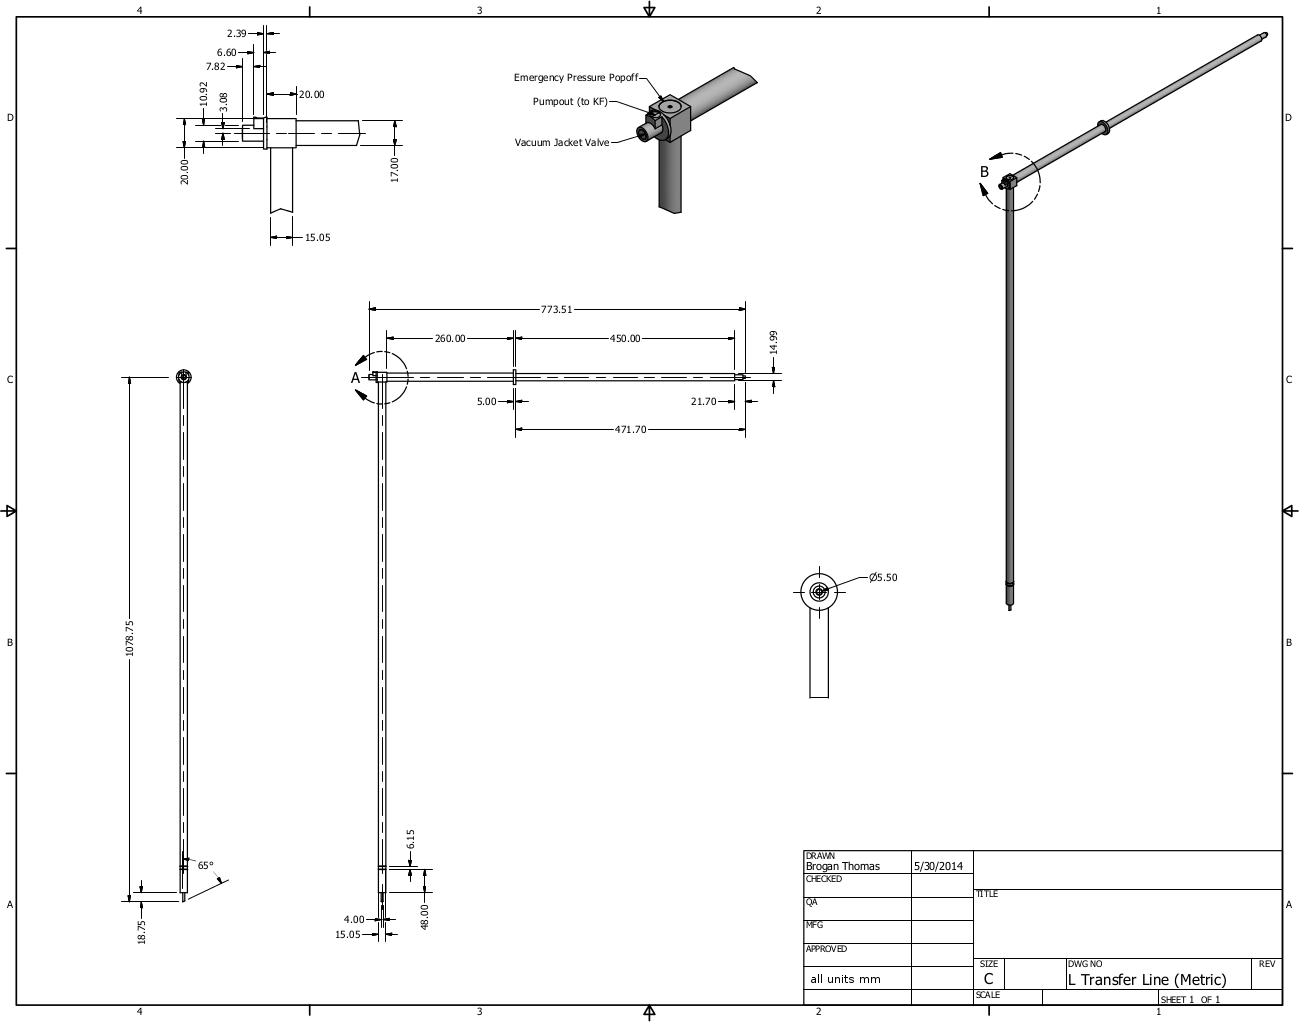
\includegraphics[width=\textwidth]{./img/LTL-drawing.png}
 \caption{Drawing of the LTL.}
 \label{fig:LTL-drawing}
\end{figure}

\begin{figure}[tbp!]
 \centering
 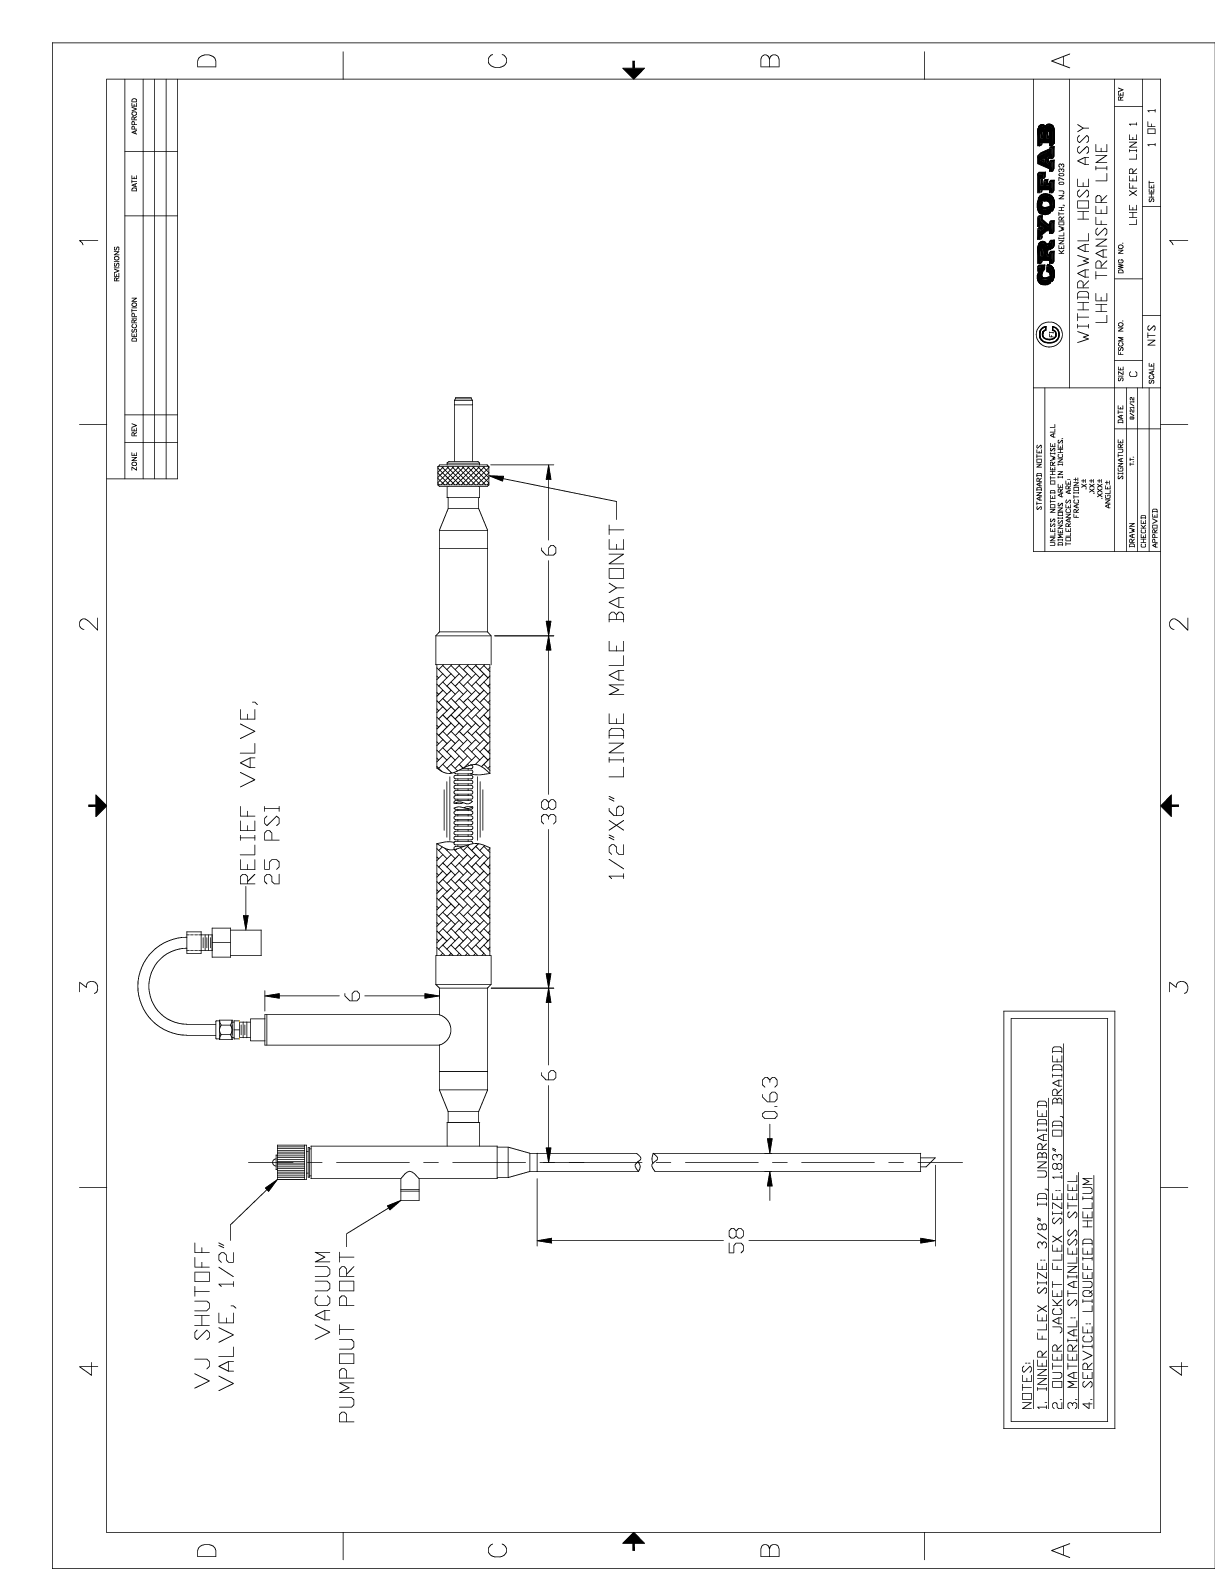
\includegraphics[width=\textwidth]{./img/500TL-drawing.png}
 \caption{Drawing of the 500TL.}
 \label{fig:500TL-drawing}
\end{figure}

\begin{figure}[tbp!]
 \centering
 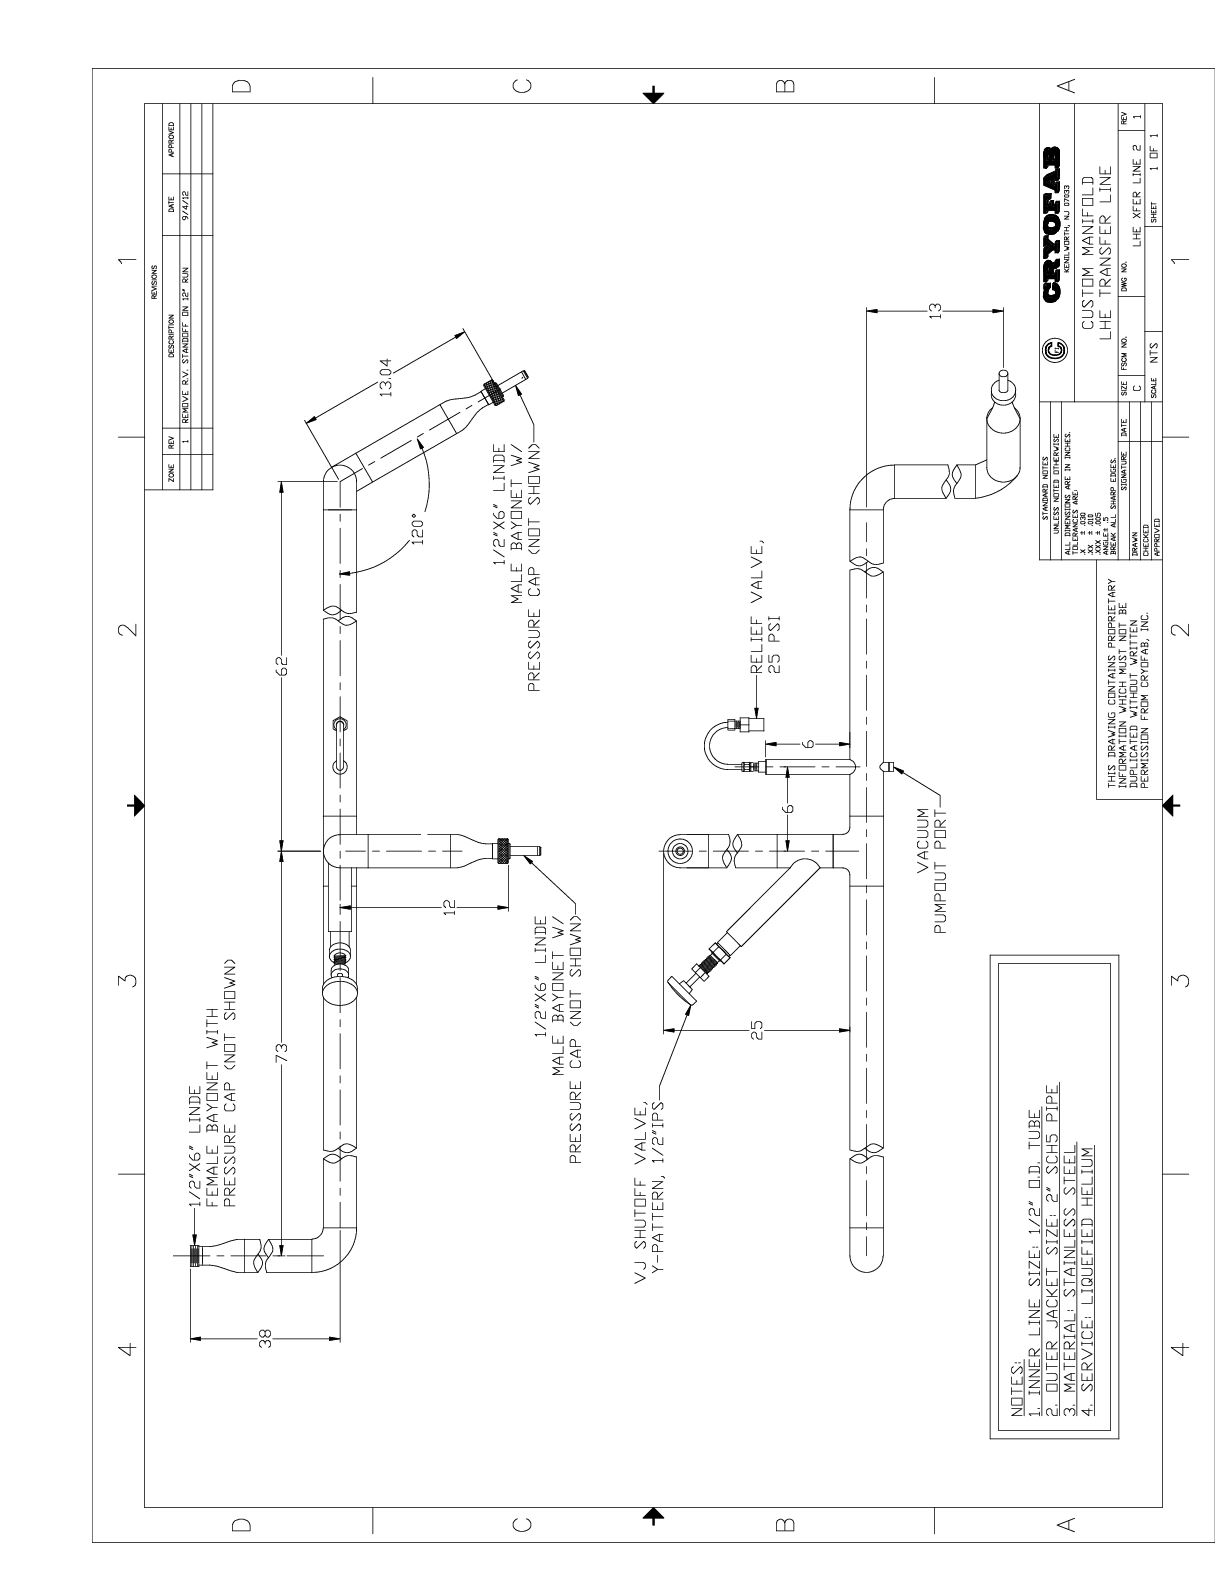
\includegraphics[width=\textwidth]{./img/WTL-drawing.png}
 \caption{Drawing of the WTL.}
 \label{fig:WTL-drawing}
\end{figure}

\begin{figure}[tbp!]
 \centering
 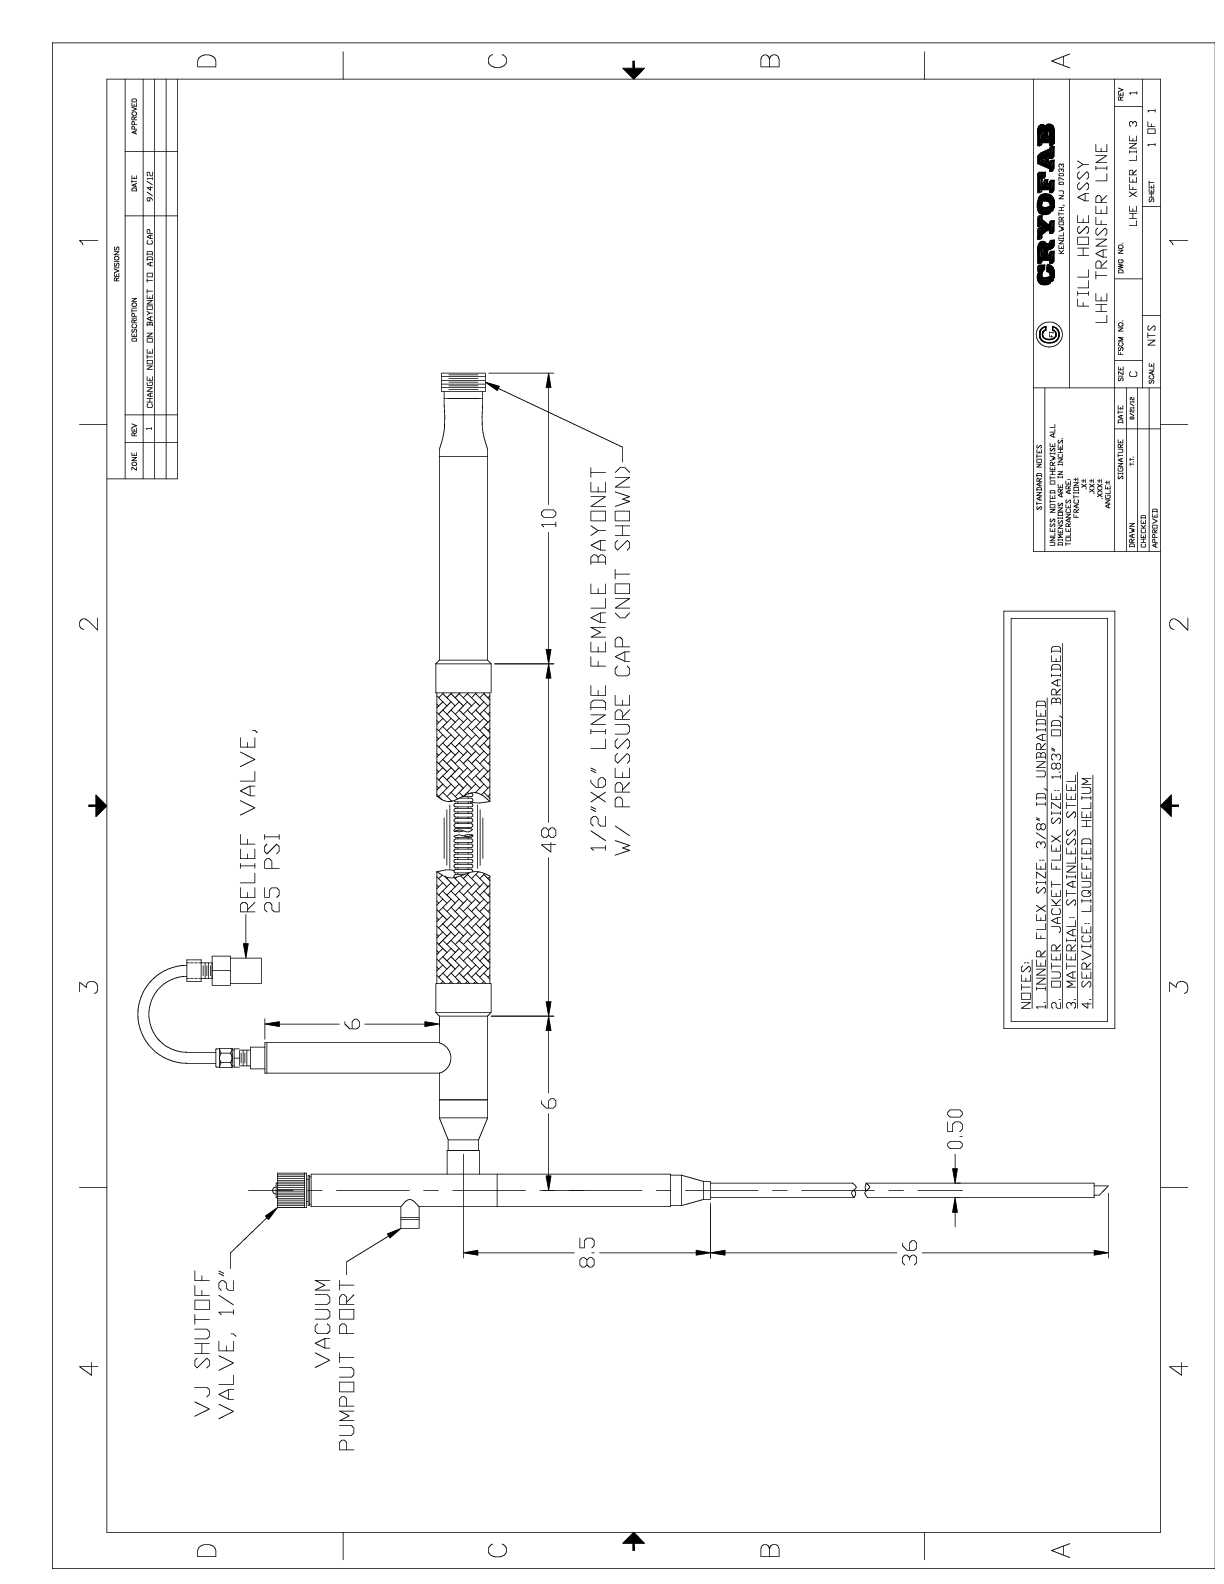
\includegraphics[width=\textwidth]{./img/MTL-drawing.png}
 \caption{Drawing of the MTL.}
 \label{fig:MTL-drawing}
\end{figure}

\begin{figure}[tbp!]
 \centering
 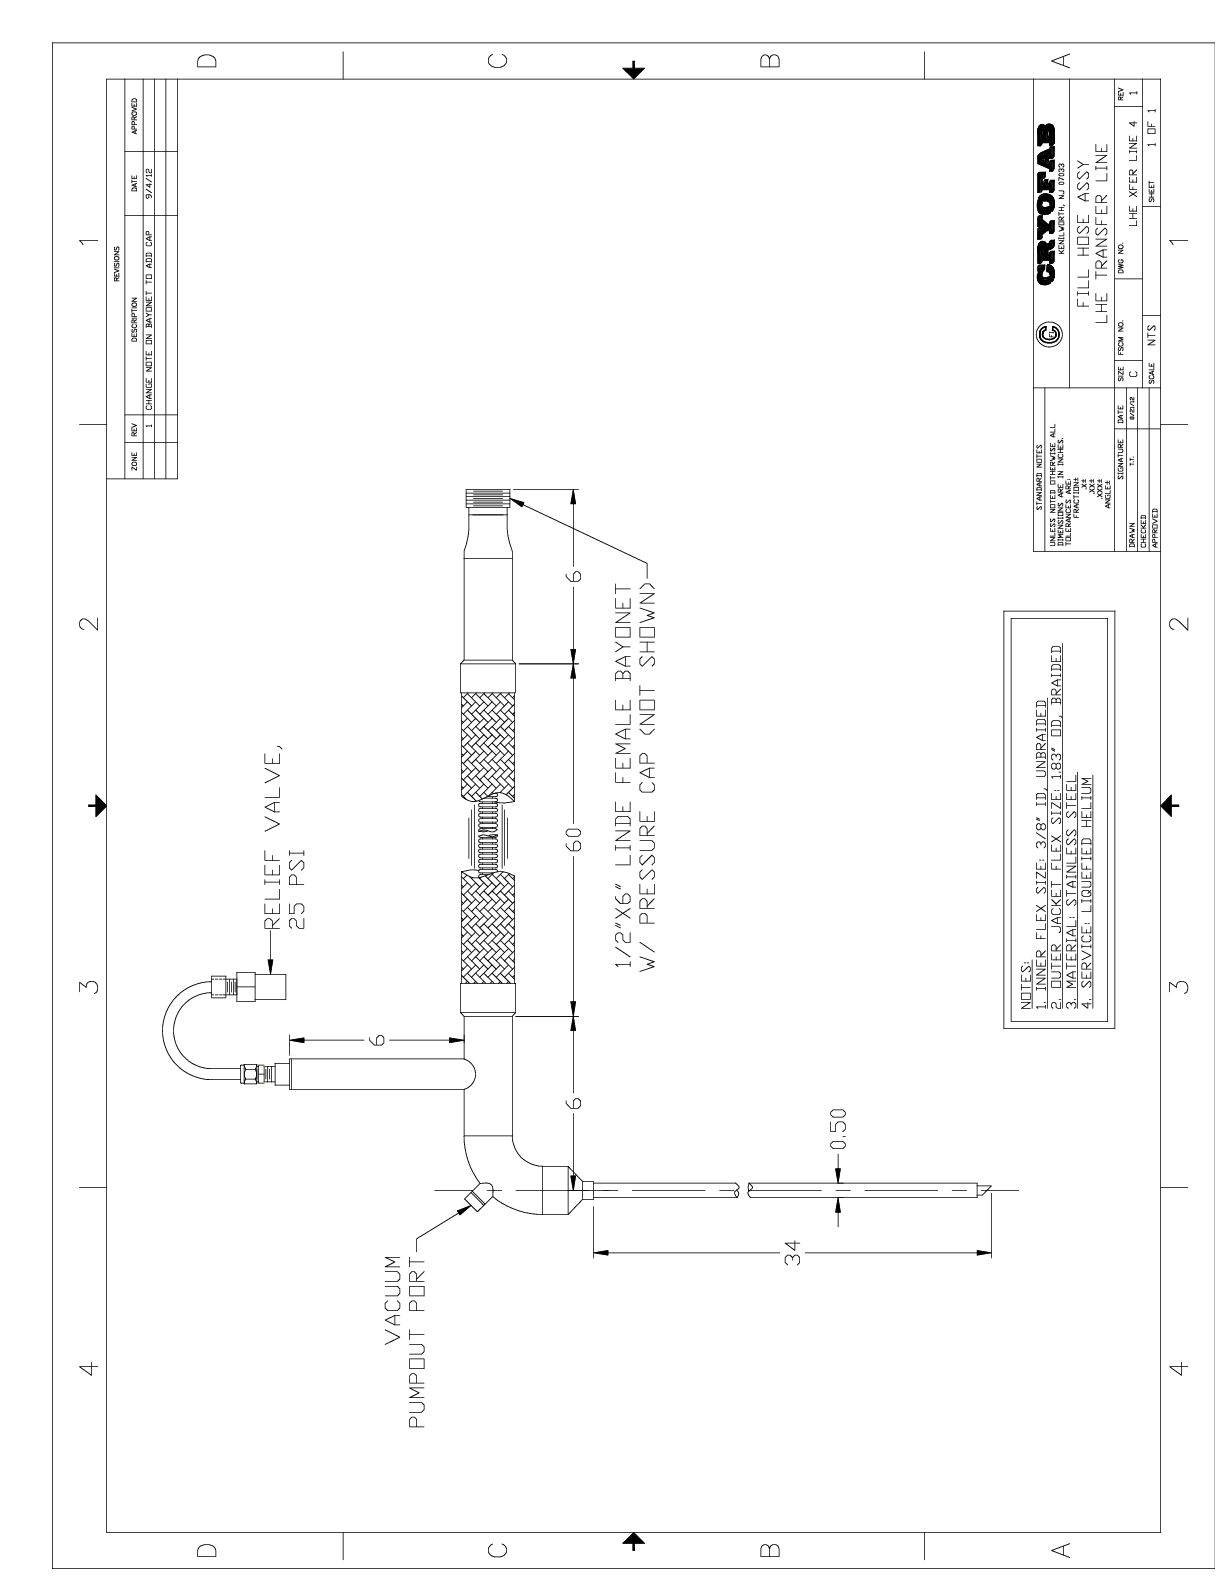
\includegraphics[width=\textwidth]{./img/100TL-drawing.png}
 \caption{Drawing of the 100TL.}
 \label{fig:100TL-drawing}
\end{figure}
\end{appendices}